\chapter{Arhitektura i dizajn sustava}
		
		\textbf{\textit{dio 1. revizije}}\\

		\textit{ Potrebno je opisati stil arhitekture te identificirati: podsustave, preslikavanje na radnu platformu, spremišta podataka, mrežne protokole, globalni upravljački tok i sklopovsko-programske zahtjeve. Po točkama razraditi i popratiti odgovarajućim skicama:}
	\begin{itemize}
		\item 	\textit{izbor arhitekture temeljem principa oblikovanja pokazanih na predavanjima (objasniti zašto ste baš odabrali takvu arhitekturu)}
		\item 	\textit{organizaciju sustava s najviše razine apstrakcije (npr. klijent-poslužitelj, baza podataka, datotečni sustav, grafičko sučelje)}
		\item 	\textit{organizaciju aplikacije (npr. slojevi frontend i backend, MVC arhitektura) }		
	\end{itemize}

	
		

		

				
		\section{Baza podataka}
			
			
		Za potrebe naše aplikacije koristimo relacijsku bazu podataka kako bismo lakše spremili i dohvaćali potrebne podatke. Baza se temelji na relacijama, tj. na tablicama definiranim imenom i atributima.
			
			\subsection{Opis tablica}
			
			
			Ova tablica sadrži sve potrebne informacije o knjigama, kao što su:
				naziv, ime i prezime autora, godina izdanja, naziv i vrstu izdavača, ISBN, broj
				izdanja, stanje i opis knjige, jezik na kojem je izdan i dostupnost. Ona je u
				One-to-One vezi s tablicom Korica preko svojeg ID-a i u One-to-Many vezi s tablicom Ponuda preko svojeg ID-a.
			
			
			\begin{longtblr}[
				label=none,
				entry=none
				]{
					width = \textwidth,
					colspec={|X[6,l]|X[6, l]|X[20, l]|}, 
					rowhead = 1,
				} %definicija širine tablice, širine stupaca, poravnanje i broja redaka naslova tablice
				\hline \SetCell[c=3]{c}{\textbf{Knjiga}}	 \\ \hline[3pt]
				\SetCell{LightGreen}ID & INT	&  Jedinstveni identificator knjige u tablici	\\ \hline
				naziv	& VARCHAR & naziv knjige   	\\ \hline 
				autor & VARCHAR & ime i prezime autora  \\ \hline 
				godina izdavanja & INT	& godina u kojoj je izdana knjiga 		\\ \hline 
				izdavac & VARCHAR	& naziv izdavača knjige 		\\ \hline 
				kategorija izdavaca & VARCHAR	& vrsta izdavača (domaći ili strani)		\\ \hline 
				ISBN & INT	& međunarodni identificator knjiga 		\\ \hline 
				broj izdanja & INT	& broj trenutnog izdanja knjige	\\ \hline 
				stanje & VARCHAR	& trenutno stanje očuvanosti knjige \\ \hline
				opis & VARCHAR	& kratki opis o radnji knjige		\\ \hline
				jezik & VARCHAR	& jezik na kojem je izdana knjiga 		\\ \hline
				dostupnost & VARCHAR & trenutna dostupnost knjige \\ \hline
				
				
			\end{longtblr}
			
			Ova tablica sadrži sve potrebne informacije o korisniku, kao što su:
				korisničko ime, lozinku korisnika, korisnikovo ime i prezime, koja je vrsta korisnika, njegov e-mail, broj mobitela i adresu. Ona je u
				u One-to-Many vezi s tablicom Ponuda preko svojeg ID-a.
			\begin{longtblr}[
				label=none,
				entry=none
				]{
					width = \textwidth,
					colspec={|X[6,l]|X[6, l]|X[20, l]|}, 
					rowhead = 1,
				} %definicija širine tablice, širine stupaca, poravnanje i broja redaka naslova tablice
				\hline \SetCell[c=3]{c}{\textbf{Korisnik}}	 \\ \hline[3pt]
				\SetCell{LightGreen}ID & INT	&  Jedinstveni identificator korisnika u tablici	\\ \hline
				korisnicko ime	& VARCHAR & korisničko ime izdavača, antikvarijata ili preprodavača  	\\ \hline 
				lozinka & VARCHAR & lozinka korisnika  \\ \hline 
				naziv korisnika & VARCHAR	& ime i prezime korisnika 		\\ \hline 
				vrsta korisnika & VARCHAR	& korisnik može biti izdavač, antikvarijat ili preprodavač 		\\ \hline 
				e-mail& VARCHAR	& e-mail korisnika		\\ \hline 
				broj mobitela & INT	& korisnikov broj mobitela		\\ \hline 
				adresa & VAR	& adresa korisnika 		\\ \hline 
				
				
			\end{longtblr}
			
			Ova tablica sadrži sve potrebne informacije o dostupnim ponudama, kao što su:
				cijena knjige i broj dostupnih knjiga. Ona je u
				u Many-to-One vezi s tablicama Korisnik i Knjiga preko ID-a od korisnika i knjige.
			\begin{longtblr}[
				label=none,
				entry=none
				]{
					width = \textwidth,
					colspec={|X[6,l]|X[6, l]|X[20, l]|}, 
					rowhead = 1,
				} %definicija širine tablice, širine stupaca, poravnanje i broja redaka naslova tablice
				\hline \SetCell[c=3]{c}{\textbf{Ponuda}}	 \\ \hline[3pt]
				\SetCell{LightGreen}ID & INT	&  Jedinstveni identificator ponude u tablici	\\ \hline
				cijena	& FLOAT & cijena u eurima po kojoj se knjiga nudi	\\ \hline 
				broj primjeraka	& INT & trenutni broj dostupnih knjiga	\\ \hline 
				\SetCell{LightBlue} ID korisnika	& INT &  Identificator korisnika iz tablice Korisnik 	\\ \hline 
				\SetCell{LightBlue} ID knjige	& INT &  Identificator knjige iz tablice Knjiga  	\\ \hline 
				
			\end{longtblr}
	       	Ova tablica sadrži slike korica knjiga. Ona je u 
				One-to-One vezi s tablicom Knjiga ID-a od knjige.
			\begin{longtblr}[
				label=none,
				entry=none
				]{
					width = \textwidth,
					colspec={|X[6,l]|X[6, l]|X[20, l]|}, 
					rowhead = 1,
				} %definicija širine tablice, širine stupaca, poravnanje i broja redaka naslova tablice
				\hline \SetCell[c=3]{c}{\textbf{Korica}}	 \\ \hline[3pt]
				\SetCell{LightGreen}ID & INT	&  Jedinstveni identificator korice u tablici	\\ \hline
				slika	& VARCHAR & Slika korice (spremljeno u bazi kao putanja do slike)	\\ \hline 
				\SetCell{LightBlue} ID knjige	& INT &  Identificator knjige iz tablice Knjiga  	\\ \hline 
				
			\end{longtblr}
			
			
			
			\subsection{Dijagram baze podataka}
			
			\begin{figure}
				\centering
				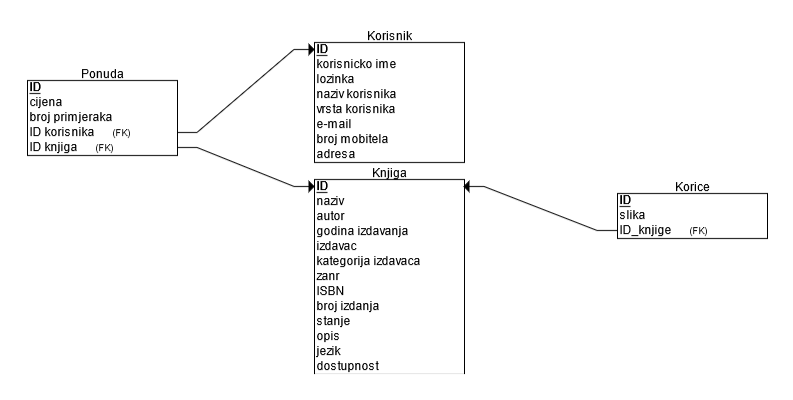
\includegraphics[width = \textwidth]{slike/Relacijska shema}
				\caption{Slika relacijske sheme}
				\label{fig:enter-label}
			\end{figure}
			
			\eject
			
		\section{Dijagram razreda}
		
			\raggedright{Razred Knjiga predstavlja jednu knjigu koja se može pronaći na stranici. Razred Neregistrirani predstavlja korisnika koji može samo pretraživati knjige. Razred registrirani predstavlja korisnika koji sustav koristi za ponudu knjiga. Izdavač, Antikvarijat i Preprodavač su razredi koji predstavljaju različite vrste registriranog korisnika. Svaki registrirani korisnik je jedna od tih tri vrste i zbog toga je razred Registrirani apstraktan. Razred Ponuda predstavlja ponudu jedne knjige. Razred VrstaKnjige predstavlja vrstu svake knjige.}\\
			
			\begin{figure}[h]
				\centering
				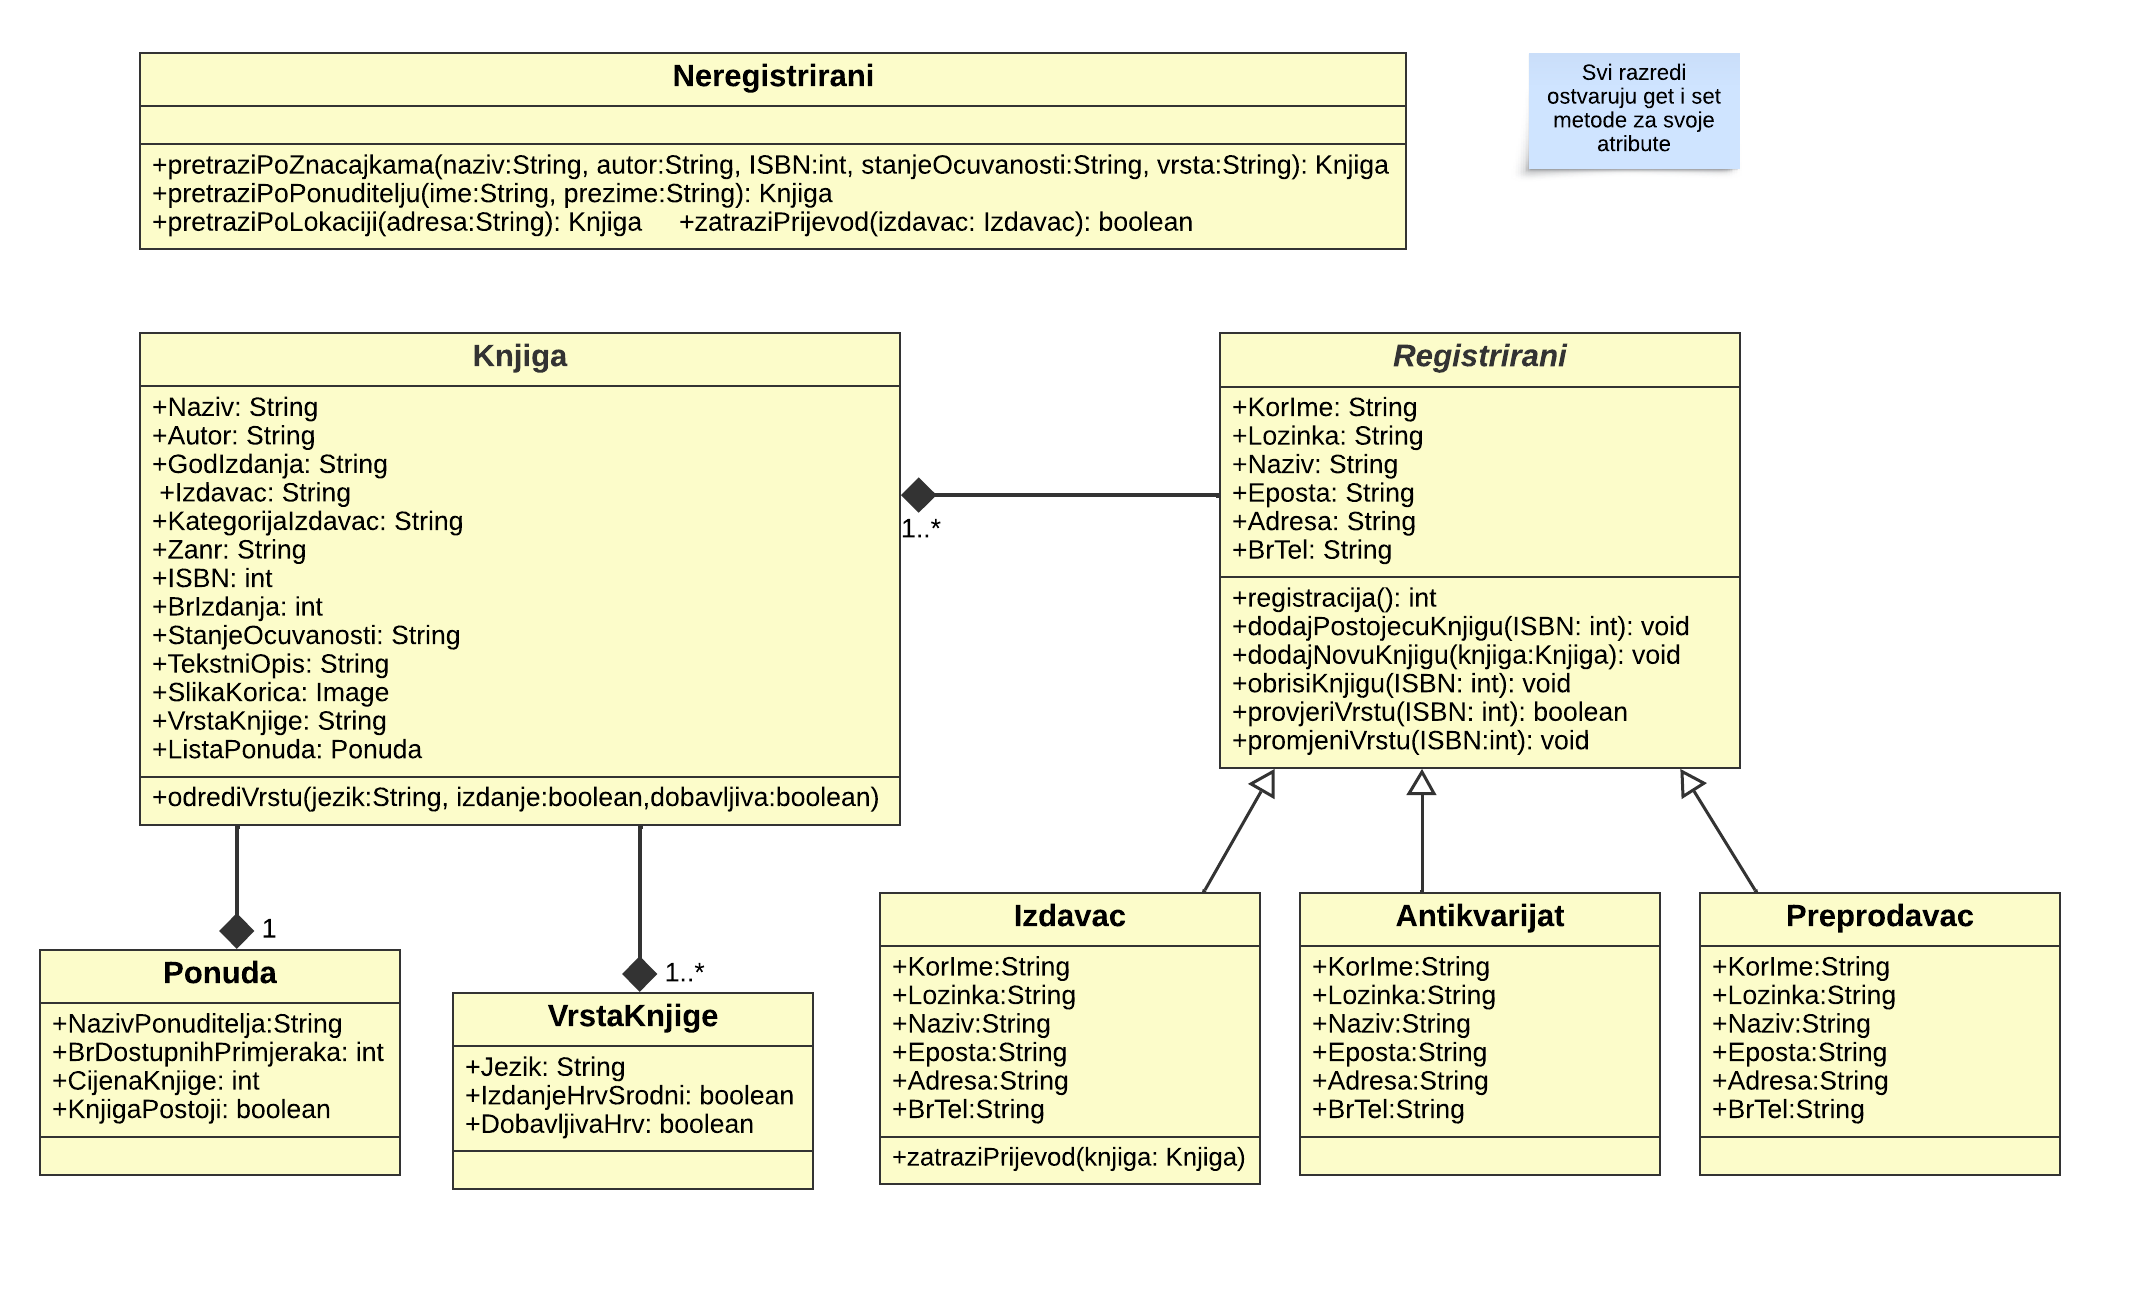
\includegraphics[width = \textwidth]{slike/dijagramKlasa.PNG}
				\caption{Dijagram razreda}
				\label{fig:enter-label}
			\end{figure}
			
			\textbf{\textit{dio 2. revizije}}\\			
			
			\textit{Prilikom druge predaje projekta dijagram razreda i opisi moraju odgovarati stvarnom stanju implementacije}
			
			
			
			\eject
		
		\section{Dijagram stanja}
			
			
			\textbf{\textit{dio 2. revizije}}\\
			
			\textit{Potrebno je priložiti dijagram stanja i opisati ga. Dovoljan je jedan dijagram stanja koji prikazuje \textbf{značajan dio funkcionalnosti} sustava. Na primjer, stanja korisničkog sučelja i tijek korištenja neke ključne funkcionalnosti jesu značajan dio sustava, a registracija i prijava nisu. }
			
			
			\eject 
		
		\section{Dijagram aktivnosti}
			
			\textbf{\textit{dio 2. revizije}}\\
			
			 \textit{Potrebno je priložiti dijagram aktivnosti s pripadajućim opisom. Dijagram aktivnosti treba prikazivati značajan dio sustava.}
			
			\eject
		\section{Dijagram komponenti}
		
			\textbf{\textit{dio 2. revizije}}\\
		
			 \textit{Potrebno je priložiti dijagram komponenti s pripadajućim opisom. Dijagram komponenti treba prikazivati strukturu cijele aplikacije.}